% Options for packages loaded elsewhere
\PassOptionsToPackage{unicode}{hyperref}
\PassOptionsToPackage{hyphens}{url}
%
\documentclass[
]{article}
\usepackage{hyphenat}
\usepackage{amsmath,amssymb}
\usepackage{iftex}
\ifPDFTeX
  \usepackage[T1]{fontenc}
  \usepackage[utf8]{inputenc}
  \usepackage{textcomp} % provide euro and other symbols
\else % if luatex or xetex
  \usepackage{unicode-math} % this also loads fontspec
  \defaultfontfeatures{Scale=MatchLowercase}
  \defaultfontfeatures[\rmfamily]{Ligatures=TeX,Scale=1}
\fi
\usepackage{lmodern}
\ifPDFTeX\else
  % xetex/luatex font selection
\fi
% Use upquote if available, for straight quotes in verbatim environments
\IfFileExists{upquote.sty}{\usepackage{upquote}}{}
\IfFileExists{microtype.sty}{% use microtype if available
  \usepackage[]{microtype}
  \UseMicrotypeSet[protrusion]{basicmath} % disable protrusion for tt fonts
}{}
\makeatletter
\@ifundefined{KOMAClassName}{% if non-KOMA class
  \IfFileExists{parskip.sty}{%
    \usepackage{parskip}
  }{% else
    \setlength{\parindent}{0pt}
    \setlength{\parskip}{6pt plus 2pt minus 1pt}}
}{% if KOMA class
  \KOMAoptions{parskip=half}}
\makeatother
\usepackage{xcolor}
\usepackage{graphicx}
\makeatletter
\def\maxwidth{\ifdim\Gin@nat@width>\linewidth\linewidth\else\Gin@nat@width\fi}
\def\maxheight{\ifdim\Gin@nat@height>\textheight\textheight\else\Gin@nat@height\fi}
\makeatother
% Scale images if necessary, so that they will not overflow the page
% margins by default, and it is still possible to overwrite the defaults
% using explicit options in \includegraphics[width, height, ...]{}
\setkeys{Gin}{width=\maxwidth,height=\maxheight,keepaspectratio}
% Set default figure placement to htbp
\makeatletter
\def\fps@figure{htbp}
\makeatother
\setlength{\emergencystretch}{3em} % prevent overfull lines
\providecommand{\tightlist}{%
  \setlength{\itemsep}{0pt}\setlength{\parskip}{0pt}}
\setcounter{secnumdepth}{-\maxdimen} % remove section numbering
\usepackage[utf8]{inputenc}
\usepackage[T1]{fontenc}
\usepackage[spanish]{babel}
\usepackage{mathptmx}
\usepackage{geometry}
\usepackage{setspace}
\usepackage{graphicx}
\usepackage{hyperref}
\usepackage{textcomp}
\DeclareUnicodeCharacter{2265}{\ensuremath{\ge}}
\DeclareUnicodeCharacter{2264}{\ensuremath{\le}}
\DeclareUnicodeCharacter{2192}{\ensuremath{\rightarrow}}
\DeclareUnicodeCharacter{00D7}{\ensuremath{\times}}
\DeclareUnicodeCharacter{2013}{--}
\DeclareUnicodeCharacter{2014}{---}
\DeclareUnicodeCharacter{00A0}{ }
\DeclareUnicodeCharacter{2248}{\ensuremath{\approx}}
\geometry{a4paper,left=4.4cm,right=4.4cm,top=5.2cm,bottom=5.2cm}
\singlespacing
\setlength{\baselineskip}{12pt}
\graphicspath{{./figures/}}
\ifLuaTeX
  \usepackage{selnolig}  % disable illegal ligatures
\fi
\IfFileExists{bookmark.sty}{\usepackage{bookmark}}{\usepackage{hyperref}}
\IfFileExists{xurl.sty}{\usepackage{xurl}}{} % add URL line breaks if available
\urlstyle{same}
\hypersetup{
  hidelinks,
  pdfcreator={LaTeX via pandoc}}

\author{}
\date{}

\begin{document}

\hypertarget{preliminary-study-for-selecting-language-models-on-local-hardware-analysis-of-the-localscore-benchmark-in-the-context-of-privacy-access-and-computational-sovereignty.}{%
\section{Local deployment of language models on heterogeneous hardware:
a decision-support framework based on hardware profiles,
interactivity, and user
practices}\label{preliminary-study-for-selecting-language-models-on-local-hardware-analysis-of-the-localscore-benchmark-in-the-context-of-privacy-access-and-computational-sovereignty.}}

Local deployment of pretrained language models responds to tensions around privacy, access, and computational sovereignty. However, pronounced hardware heterogeneity makes it difficult to determine which models are viable in each context and what user experience can be expected. This paper reports progress toward a decision-support tool for local deployment under diverse hardware constraints.

The contribution is organized in three strands: (i) identifying relevant characteristics of hardware, language models, and user profiles; (ii) proposing operational categories for each of these components; and (iii) articulating these categories using empirical evidence to guide model selection.

Methodologically, we analyze 1,556 runs from the public LocalScore benchmark and complement them with exploratory interviews with three key informants (teacher, social science researcher, developer). We introduce an interactivity criterion based on silent reading speed in Spanish (Brysbaert, 2019), linking technical metrics to concrete usage experiences. In our sample, CPU-only configurations sustain conversational use for 1--4B models (M2), while 8--16B models (M4) fall predominantly into batch mode; with mid-to-high-end GPUs, M4 becomes viable for fluid interaction.

Building on these findings, we propose a preliminary framework that, given a hardware profile and a user or practice type, suggests viable model size ranges and the expected usage experience, reducing adoption friction without requiring specialized technical knowledge.

\textbf{Keywords:} language models, local inference,
resource-constrained hardware, computational sovereignty, benchmark.

\begin{center}\rule{0.5\linewidth}{0.5pt}\end{center}

\hypertarget{estudio-preliminar-para-la-selecciuxf3n-de-modelos-de-lenguaje-en-hardware-local-anuxe1lisis-del-benchmark-localscore-en-el-marco-de-privacidad-acceso-y-soberanuxeda-computacional.}{%
\section{Despliegue local de modelos de lenguaje en hardware heterogéneo:
un marco de apoyo a la decisión basado en perfiles de hardware,
interactividad y prácticas de
usuario}\label{estudio-preliminar-para-la-selecciuxf3n-de-modelos-de-lenguaje-en-hardware-local-anuxe1lisis-del-benchmark-localscore-en-el-marco-de-privacidad-acceso-y-soberanuxeda-computacional.}}

La implementación local de modelos de lenguaje preentrenados surge como respuesta a tensiones de privacidad, acceso y soberanía computacional. Sin embargo, la marcada heterogeneidad del hardware disponible dificulta determinar qué modelos son viables en cada contexto y qué experiencia de uso puede esperarse. Este trabajo presenta avances hacia el desarrollo de una herramienta orientada a acompañar la toma de decisiones sobre despliegue local bajo distintas restricciones de hardware.

La contribución se organiza en tres ejes: (i) la identificación de características relevantes del hardware, de los modelos de lenguaje y de los perfiles de usuario; (ii) la propuesta de categorías operativas para cada uno de estos tres componentes; y (iii) la articulación entre dichas categorías a partir de evidencia empírica, con el fin de orientar la selección de modelos.

Metodológicamente, se analizan 1556 ejecuciones del benchmark público LocalScore y se complementan con entrevistas exploratorias a tres informantes clave (docente, investigador social y desarrollador). Asimismo, se introduce un criterio de interactividad basado en la velocidad de lectura en español (Brysbaert, 2019), que permite vincular métricas técnicas con experiencias de uso concretas. En la muestra, en configuraciones CPU-only los modelos de 1--4B (M2) sostienen uso conversacional, mientras que los de 8--16B (M4) caen predominantemente en modo batch; con GPU media/alta, M4 se vuelve viable para interacción fluida.

A partir de los hallazgos empíricos, se propone un framework preliminar que, dado un perfil de hardware y un tipo de usuario o práctica, sugiere rangos de tamaño de modelo viables y la experiencia de uso esperable, reduciendo la fricción de adopción sin exigir conocimiento técnico especializado.

\textbf{Palabras clave:} modelos de lenguaje, inferencia local, hardware
de recursos limitados, soberanía computacional, benchmark.

\begin{center}\rule{0.5\linewidth}{0.5pt}\end{center}

\hypertarget{introducciuxf3n}{%
\subsection{1. Introducción}\label{introducciuxf3n}}

Un modelo de lenguaje (LM) es un sistema entrenado para modelar y generar texto. Hoy los más utilizados son los Large Language Models (LLMs), redes neuronales que priorizan escala para capturar capacidades emergentes, mientras que los Small Language Models (SLMs) se definen operativamente por su adecuación a tareas específicas bajo restricciones de cómputo y memoria (Wang et al., 2025). La adopción masiva de servicios de LLM en la nube introduce tensiones persistentes en tres dimensiones:

\begin{itemize}
    \item Privacidad: en entornos como la docencia, la investigación social y el desarrollo de software, los datos de trabajo —código, documentos, materiales de estudiantes, transcripciones— frecuentemente no pueden compartirse con terceros.
    \item Acceso: el modelo predominante de IA como servicio implica costos por uso, límites de tokens y dependencia de conectividad, lo que excluye a usuarios individuales, instituciones educativas y organizaciones con recursos limitados que podrían beneficiarse de estas herramientas.
    \item Soberanía computacional: universidades, sistemas educativos y empresas que adoptan servicios cloud de IA delegan el control sobre su infraestructura, sus datos y los modelos que utilizan, sin posibilidad real de auditoría ni autonomía operativa.
\end{itemize}

La ejecución local de LLMs se presenta como una respuesta concreta a estas tres tensiones. Sin embargo, incluso cuando existen modelos abiertos disponibles, su adopción efectiva se ve condicionada de forma determinante por capacidades de hardware heterogéneas y por la falta de guía sistemática para orientar esa adopción. Este trabajo avanza en la construcción de un framework de selección de modelos para despliegue local, orientado por la pregunta: ¿qué modelos y configuraciones resultan adecuados para un perfil de hardware dado y un tipo de uso específico?

Este artículo presenta avances preliminares de una investigación doctoral sobre despliegue de LLMs en hardware limitado. A partir del análisis de 1556 ejecuciones del benchmark público LocalScore y de entrevistas exploratorias con tres informantes clave, realizamos cuatro contribuciones:

\begin{enumerate}
    \item Perfiles de hardware (H): una tipificación operativa de clases de equipo que permite a usuarios no especializados caracterizar su hardware en relación con el uso de LLMs.
    \item Perfiles de modelo (M): una segmentación por tamaño de parámetros que discrimina demanda de memoria y throughput en inferencia local.
    \item Criterio de interactividad: una categorización de experiencia de uso (batch, interactivo mínimo, interactivo fluido) anclada en la velocidad de lectura promedio en español (Brysbaert, 2019), que permite predecir si una configuración H×M va a ser usable de forma conversacional antes de descargar el modelo.
    \item Framework preliminar de selección: una síntesis de los resultados cuantitativos y cualitativos en lineamientos operativos que, dado un perfil de hardware, indican qué rangos de modelo son viables y qué experiencia de uso esperar (Tabla 1).
\end{enumerate}

El resto del artículo se organiza en seis secciones. §2 contextualiza los SLMs y las técnicas de optimización, e identifica el vacío de estudios sistemáticos para hardware de consumo. §3 construye las variables del marco (fuente LocalScore; perfiles H y M; criterio de experiencia/interactividad como puente entre métricas y uso). §4 caracteriza la viabilidad técnica en la muestra mediante el cruce H×M×régimen de experiencia sobre 1556 corridas. §5 aporta requisitos de uso a partir de tres entrevistas y su traducción a demandas sobre H×M. §6 articula dimensiones en lineamientos y tabla del marco preliminar. §7 identifica las limitaciones y los próximos pasos.

\hypertarget{trabajos-relacionados}{%
\subsection{2. Trabajos relacionados}\label{trabajos-relacionados}}

Los LLMs de gran escala suelen requerir uso vía cloud/API por su demanda computacional: por ejemplo, Llama 3.1 405B requiere aproximadamente 202,5 GB de memoria GPU en precisión int4 (Wang et al., 2025). Este modelo de despliegue plantea los problemas de privacidad, acceso y soberanía descritos en §1. Como alternativa, los SLMs se definen no solo por cantidad de parámetros, sino por su capacidad de ejecutar tareas especializadas dentro de restricciones de recursos: el límite inferior es el tamaño mínimo que exhibe habilidades emergentes para una tarea, y el superior es el máximo manejable bajo las condiciones de hardware disponibles (Wang et al., 2025). Este trabajo opera en ese espacio: analiza modelos de distintos tamaños ejecutados en hardware de consumo heterogéneo, y busca identificar qué combinaciones resultan viables para uso conversacional — es decir, qué modelos pueden funcionar efectivamente como SLMs en contextos de despliegue local real.

Los trabajos existentes sobre desempeño de LLMs, como Pope et al. (2022), desarrollan modelos analíticos para optimizar inferencias a escala de datacenter — modelos de 8B a 540B parámetros en hardware especializado. Este trabajo aborda el problema inverso: dado hardware de consumo heterogéneo y preexistente, ¿qué modelos resultan viables para uso conversacional?

En cuanto a técnicas de optimización, la cuantización permite reducir el tamaño de los modelos con impacto limitado en precisión; la evidencia reciente indica que 3-4 bits constituye un balance práctico para despliegue en entornos con recursos limitados (Wang et al., 2025), y este rango domina la muestra analizada: el 87\% de las ejecuciones corresponde a Q4\_K\_Medium. Esto implica que los patrones del cruce H×M reflejan principalmente diferencias por tamaño de modelo y perfil de hardware, no por cuantización — incorporar esa dimensión requiere mayor diversidad en la base y queda como trabajo futuro. Otras técnicas como mixture-of-experts (MoE) aceleran el cómputo pero no reducen los requerimientos de memoria para cargar el modelo (Yi et al., 2023), por lo que su impacto en hardware de consumo es más limitado y no están representadas en la muestra actual.

Sin embargo, estos trabajos abordan técnicas y taxonomías de modelos sin cruzar datos de rendimiento en hardware real con necesidades de uso concretas. Este trabajo aporta ese cruce: a partir de 1556 ejecuciones reales de LocalScore, introduce un criterio de interactividad anclado en la velocidad de lectura en español (Brysbaert, 2019) para traducir tokens/segundo en experiencia de usuario percibida.

\hypertarget{benchmark-y-definiciones}{%
\subsection{3. Metodología: construcción de variables (H, M, experiencia)}\label{benchmark-y-definiciones}}

Las variables que siguen son las del marco preliminar de selección: hacen comparables las corridas del benchmark y permiten expresar decisiones en términos comprensibles para usuarios sin formación técnica especializada. Esta sección define la fuente de datos (LocalScore), los perfiles operativos de hardware (H) y modelo (M), y un criterio de experiencia de uso (batch, interactivo mínimo, interactivo fluido) que funciona como lenguaje común entre la dimensión técnica y la práctica del usuario.

\hypertarget{localscore-como-benchmark-y-fuente-de-datos}{%
\subsubsection{3.1 Fuente de datos: LocalScore}\label{localscore-como-benchmark-y-fuente-de-datos}}

LocalScore es una herramienta open source de benchmarking orientada a
medir rendimiento de inferencia de modelos de lenguaje sobre hardware
específico y publicar resultados en una base pública de corridas para
comparación entre equipos (Mozilla AI, s.f.). Mide tres métricas
principales: 
\begin{itemize}
    \item avg\_prompt\_tps: velocidad de procesamiento de prompts en token/segundo,
    \item avg\_gen\_tps: velocidad promedio de generación en tokens/segundo
    \item avg\_ttft\_ms: tiempo promedio entre el envío y la respuesta del primer token.
\end{itemize}

Estas métricas corresponden a las fases de prefill (procesamiento de tokens de entrada) y decode (generación autoregresiva de tokens de salida) descritas en Pope et al. (2022) para inferencia de Transformers, aquí medidas sobre hardware de consumo heterogéneo mediante LocalScore en lugar de aceleradores de datacenter.

En este trabajo usamos cada ejecución de este benchmark como unidad de análisis,
comprendida como la ejecución del benchmark en un hardware particular,
con un modelo específico dando un resultado de métrica. Para analizar el
rendimiento con hardware y modelo utilizamos avg\_gen\_tps, relevante
para prácticas conversacionales donde la velocidad de respuesta puede
cortar el flujo.

Los datos corresponden a un dump público de LocalScore tomado el
24-09-2025 constando de 1556 ejecuciones del benchmark.

\hypertarget{perfiles-de-hardware-h}{%
\subsubsection{3.2 Perfiles de hardware
(H)}\label{perfiles-de-hardware-h}}

Los perfiles de hardware son una tipificación operativa de
\textbf{clases de equipo} para uso local de LLM (RAM en \textbf{solo
CPU} y VRAM en \textbf{GPU}, más H7 para señalar
\textbf{servidor/datacenter}) Definimos los siguientes perfiles: 
\textbf{solo CPU} --- 
\begin{itemize}
    \item H0: RAM \textless4 GB;
    \item H1: {[}4, 8) GB;
    \item H2: {[}8, 16) GB;
    \item H3: ≥16 GB.
\end{itemize}
\textbf{GPU} --- 
\begin{itemize}
    \item H4: VRAM \textless8 GB;
    \item H5: {[}8, 24) GB;
    \item H6: VRAM ≥24 GB;
    \item H7: \textbf{acelerador/datacenter} --- identificado como servidor en el dump (independiente de los cortes anteriores).
\end{itemize}
Se sostiene H0 como perfil de interés por los objetivos del estudio aunque la muestra
contiene solo 6 ejecuciones. Los perfiles no pretenden censar población ni capturar todo el hardware, sino caracterizar escenarios de despliegue local relevantes para el estudio.

\hypertarget{perfiles-de-modelo-m}{%
\subsubsection{3.3 Perfiles de modelo (M)}\label{perfiles-de-modelo-m}}

Los perfiles M se definen por número de parámetros, variable que más
discrimina demanda de memoria y throughput en inferencia local. La
cuantización queda controlada implícitamente por la composición de la
muestra: el 87\% de las ejecuciones corresponde a Q4\_K-Medium, por lo
que los patrones del cruce H×M reflejan principalmente diferencias por
tamaño y hardware. Esta homogeneidad limita la generalización a otras
cuantizaciones; incorporar esa dimensión requiere mayor diversidad en la
base y queda como trabajo futuro (§7).

Tipificamos tamaño de modelo por cantidad de parámetros en cinco
perfiles: M1:\textless1B, M2: {[}1--4)B, M3:{[}4--8)B, M4:{[}8--16)B,
M5:\textgreater=16B.

\hypertarget{categoruxedas-de-performance-experiencia-de-uso}{%
\subsubsection{3.4 Categorías de performance (experiencia de
uso)}\label{categoruxedas-de-performance-experiencia-de-uso}}

Para aproximar si una corrida se comporta como interactiva o como batch,
usamos avg\_gen\_tps como proxy de la velocidad a la que el usuario
recibe texto en streaming. Según Brysbaert (2019), la velocidad promedio
de lectura silenciosa en español es de 278 palabras por minuto (ppm). Dado que en ese idioma la relación es de aproximadamente 1,7 tokens por palabra, podemos
estimar ppm ≈ (tps / 1,7) × 60; así, 10 tok/s corresponde a
\textasciitilde350 ppm, valor que ya supera la velocidad de lectura
promedio. 

A diferencia de umbrales definidos para infraestructura de servidor —como el rango 20–50 tok/s de MLPerf, derivado de plataformas cloud—, este trabajo adopta la velocidad de lectura como criterio mínimo por una razón funcional: en el contexto de hardware limitado, el umbral relevante no es la fluidez óptima sino el punto a partir del cual el usuario puede leer la respuesta sin esperar que el modelo termine de generarla. Los 10 tok/s representan ese umbral mínimo; los 25 tok/s operacionalizan la fluidez como generación notablemente más rápida que la lectura.

Sobre esta base definimos tres categorías heurísticas: Batch
(\textless10 tok/s), interactivo mínimo (10--25 tok/s) e interactivo
fluido (≥25 tok/s). Los cortes son un punto de partida operativo para
segmentar regímenes de experiencia, no un estándar validado, y no
sustituyen otras dimensiones relevantes (p.~ej. latencia inicial/TTFT,
tipo de tarea o calidad de salida), que planeamos incorporar en trabajo
futuro.

\hypertarget{resultados-cuantitativos}{%
\subsection{4. Viabilidad técnica según H×M (evidencia LocalScore)}\label{resultados-cuantitativos}}

Esta sección aporta \textbf{insumos de viabilidad técnica} al marco preliminar: sobre la base de LocalScore, caracteriza qué combinaciones H×M resultan plausibles en la muestra en términos de régimen de generación (batch/interactivo), según las definiciones de §3. A continuación se aplican esas definiciones a las 1556 corridas del benchmark. Primero se describe la distribución de la muestra por perfil de hardware y modelo, y luego se presenta el cruce H×M×régimen de experiencia que constituye la base empírica del framework.

\hypertarget{distribuciuxf3n-de-hardware-y-modelos}{%
\subsubsection{4.1 Distribución de hardware y
modelos}\label{distribuciuxf3n-de-hardware-y-modelos}}

La muestra se concentra en perfiles medios/altos (H3, H5 y H6), y tiene
menor cobertura en extremos (H1, H4, H7), condicionando robustez en
celdas H×M con baja muestra. Los modelos presentan distribución bimodal
por tamaño y concentración en pocas familias; por ello, las conclusiones
más sólidas del cruce se ubican en las bandas con mayor volumen (M2 y
M4).

\hypertarget{cruce-hardware-tamauxf1o-de-modelo-performance}{%
\subsubsection{4.2 Cruce hardware × tamaño de modelo ×
performance}\label{cruce-hardware-tamauxf1o-de-modelo-performance}}

Reportamos el cruce H1--H7 (excluyendo H0) para evitar que una celda con
muy baja cobertura distorsione la lectura agregada. El cruce exhibe dos
patrones: 
\begin{itemize}
    \item (i) quiebre en M4 (8B--16B): H3--M4 es 80.9\% batch (148/183), mientras que en GPU H5--M4 es 66.4\% fluido (160/241) y H6--M4 67.8\% fluido (137/202);
    \item (ii) robustez en M2 (1B-- 4B): H3--M2 alcanza 96.0\% interactivo total (214/223) y 73.5\% fluido (164/223), y en H5/H6 el fluido ronda 94.6\%.
\end{itemize}

\textbf{Resultado clave:} estos resultados permiten que el framework tome una
primera decisión ``de viabilidad'' por perfil de hardware: qué rangos de
tamaño (M) pueden aspirar a modo batch vs.~interactivo.

\begin{figure}
\centering
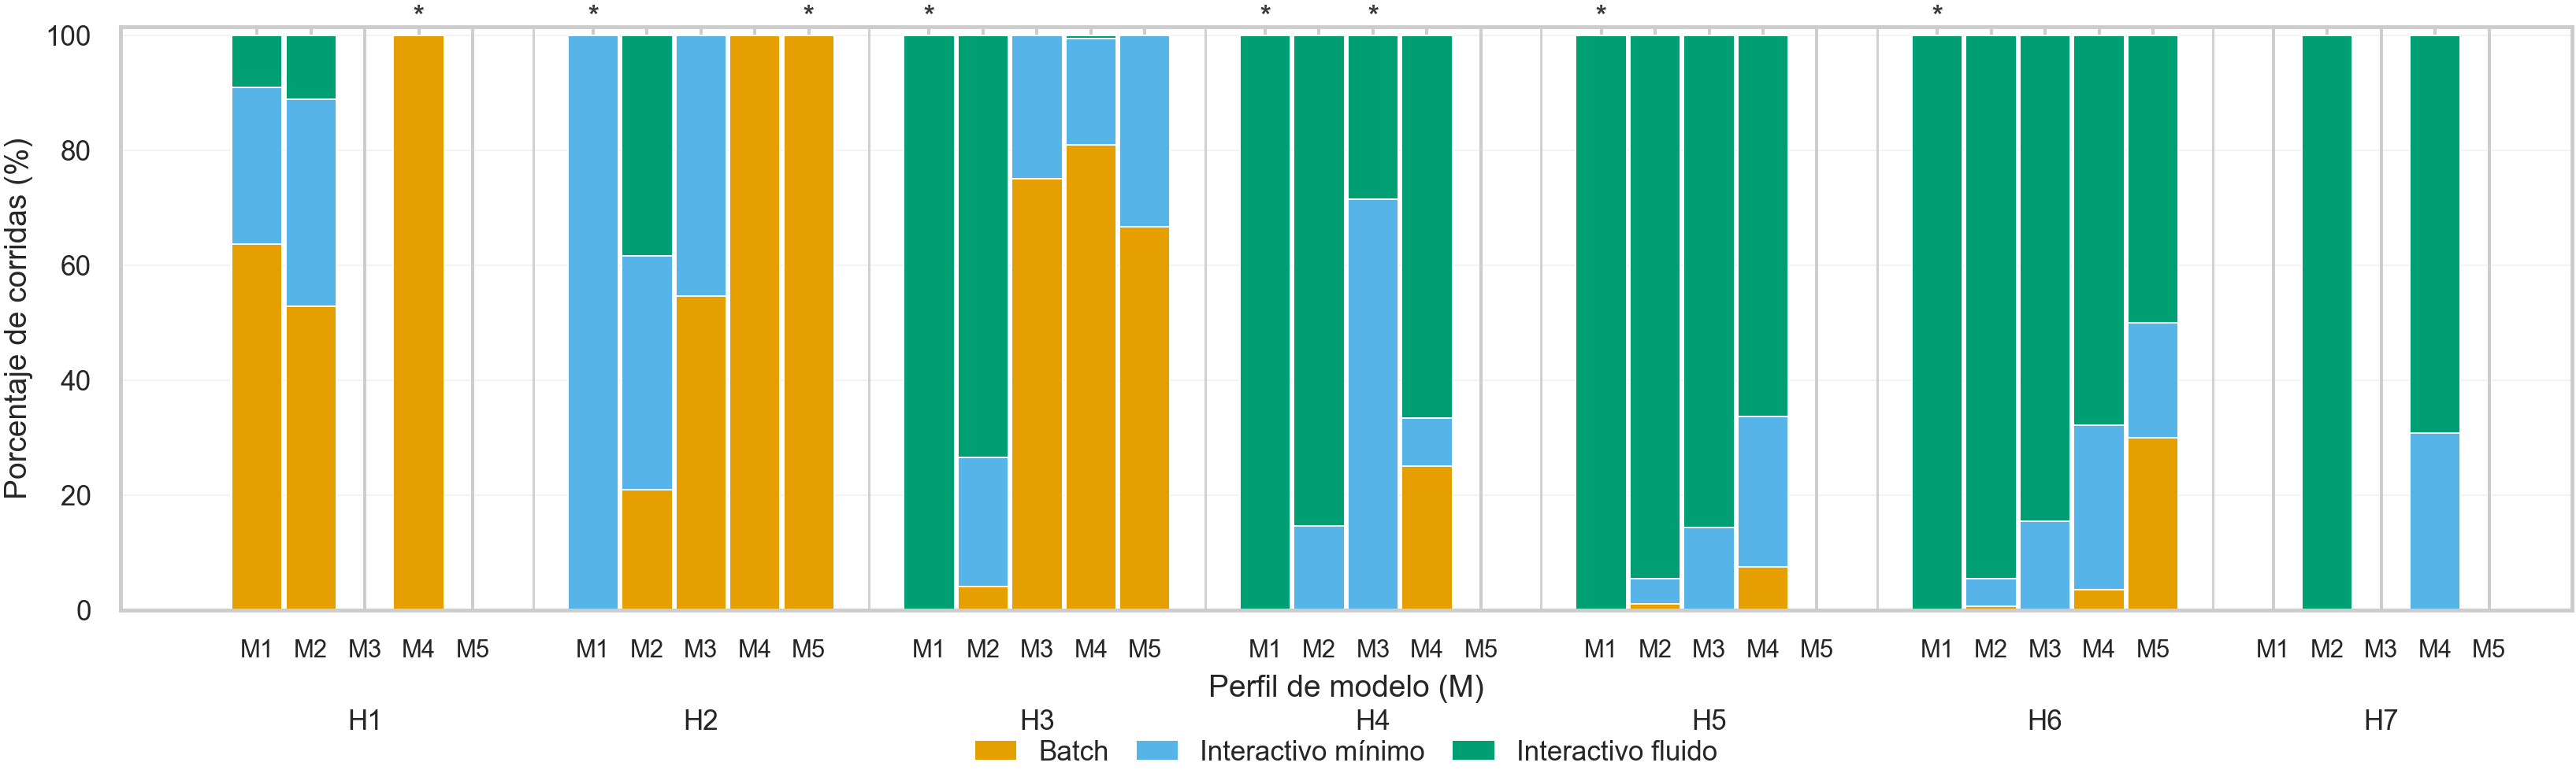
\includegraphics{figures/fig03_hardware_model_perf_percent_clean.png}
\caption{Hardware × tamaño de modelo × performance (\% por
H×M).}
\end{figure}

\emph{Nota: el asterisco (*) indica combinaciones H×M con n\textless10
corridas.}

Cuando la práctica exige privacidad/soberanía y el hardware cae en zonas
CPU-only con baja interactividad (p.~ej. M4), el cruce sugiere
considerar despliegue local en GPU/servidor institucional o ajustar a
tamaños M más pequeños.

\hypertarget{resultados-cualitativos}{%
\subsection{5. Requisitos de uso y perfiles de usuario}\label{resultados-cualitativos}}

Esta sección aporta \textbf{insumos de adecuación al uso}: identifica prácticas, restricciones y trade-offs ---en particular, demandas de interactividad, tolerancia a la latencia, costo del error y sensibilidad de los datos--- que condicionan qué configuraciones resultan aceptables más allá de la viabilidad técnica del §4. Se realizaron tres entrevistas exploratorias semi-estructuradas, grabadas, transcriptas y sistematizadas, de aproximadamente una hora cada una. Los casos fueron seleccionados por criterio de pertinencia teórica: cada perfil representa un tipo de práctica con características distintivas en relación al objeto de estudio. Los docentes universitarios trabajan con datos estudiantiles sensibles y materiales pedagógicos que frecuentemente no pueden compartirse con servicios externos. Los investigadores de ciencias sociales producen y analizan grandes volúmenes de datos cualitativos — entrevistas, transcripciones, documentos — que antes requerían técnicas de análisis más limitadas y que hoy son candidatos naturales al procesamiento con LLMs locales. Los desarrolladores y SREs operan con código propietario e infraestructura interna donde la privacidad y la soberanía son requisitos operativos, no preferencias. Los tres perfiles son además informantes clave: tienen conocimiento profundo de las prácticas, herramientas y restricciones de sus respectivos campos. No se busca generalización estadística sino una exploración prospectiva que permita orientar los objetivos del trabajo y anclar el cruce cuantitativo en necesidades de uso reales.

\hypertarget{caso-docente-universidad.}{%
\subsubsection{5.1 Caso docente
(universidad).}\label{caso-docente-universidad.}}

\textbf{Prácticas prioritarias:} planificación y actualización de
programas; producción de materiales (Moodle/recursos); consultas FAQ;
preguntas de autoevaluación; apoyo con bibliografía (RAG).
\textbf{Hardware del entorno:} laboratorios institucionales con 8 GB RAM sin GPU (H2); dispositivo personal no detallado; la práctica actual depende de servicios cloud.
\textbf{Trade-offs:} tolera batch para materiales; error/alucinación
crítico en evaluación; sensibilidad alta a datos estudiantiles.

\hypertarget{caso-investigador-social.}{%
\subsubsection{5.2 Caso investigador
social.}\label{caso-investigador-social.}}

\textbf{Prácticas:} escritura/revisión; análisis cualitativo con
trazabilidad; transcripción (Whisper); instrumentos;
evaluación/revisión.
\textbf{Hardware del campo:} promedio limitado (8 GB RAM, sin GPU, H2); el informante es outlier con GPU (GTX 1060, 3 GB VRAM, H4).
\textbf{Trade-offs:} riesgo crítico de alucinación
bibliográfica; necesidad de verificación; hardware del campo tensiona ejecución local.

\hypertarget{caso-desarrolladorsre.}{%
\subsubsection{5.3 Caso
desarrollador/SRE.}\label{caso-desarrolladorsre.}}

\textbf{Prácticas:} migraciones masivas (p.~ej. Ansible); refactors;
tests; documentación/onboarding; scripting/diagnóstico.
\textbf{Hardware típico:} notebooks personales heterogéneas (≥16 GB RAM, CPU-only, H3); servidor compartido de la cooperativa con GPU de alta gama (2× RTX 5090, H6).
\textbf{Trade-offs:} costo de error alto; preferencia por ejecución
local por privacidad/soberanía; acepta batch para tareas largas con
verificabilidad.

\hypertarget{traducciuxf3n-de-pruxe1cticas-a-muxe9tricas-y-perfiles-hm}{%
\subsubsection{5.4 Traducción de prácticas a métricas y perfiles
H×M}\label{traducciuxf3n-de-pruxe1cticas-a-muxe9tricas-y-perfiles-hm}}

Para conectar los hallazgos cualitativos con el cruce cuantitativo,
traducimos cada práctica a una métrica observable de desempeño:
velocidad de generación (avg\_gen\_tps). En línea con §3.4, usamos tres
regímenes por avg\_gen\_tps (batch \textless10 tok/s; interactivo mínimo
10--25; fluido ≥25) y mapeamos esos requerimientos a celdas H×M del
benchmark (§4.2).

\begin{itemize}
\tightlist
\item
  \textbf{Docente:} consultas y apoyo en clase requieren interactividad;
  producción de materiales admite batch. Esto favorece M2 en H3 y
  desaconseja asumir M4 interactivo en CPU-only.
\item
  \textbf{Investigación social:} con hardware más restringido (p.~ej., 8
  GB sin GPU), la interactividad se concentra en M1--M2; el alto costo
  del error exige verificación humana además del criterio de
  rendimiento.
\item
  \textbf{Desarrollo/SRE:} iteración rápida (diagnóstico/refactor)
  demanda interactividad; tareas largas verificables pueden correr en
  batch. M4 se vuelve más consistente con GPU (H4+), mientras en
  CPU-only conviene priorizar M2.
\end{itemize}

\hypertarget{sintesis-framework}{%
\subsection{6. Articulación de dimensiones y propuesta de marco preliminar}\label{sintesis-framework}}

Aquí se \textbf{integran} los insumos de viabilidad técnica (§4) y los de adecuación al uso (§5) en lineamientos operativos y en una síntesis tabular del marco preliminar. Los resultados cuantitativos y cualitativos convergen en una primera versión del framework de selección de modelos para despliegue local. El framework toma como entrada el perfil de hardware del usuario (H) y produce como salida el rango de tamaño de modelo (M) viable, el régimen de experiencia esperado y las advertencias de despliegue relevantes. El cruce H×M por régimen de generación (§4.2) aporta la base empírica de desempeño, y la evidencia cualitativa (§5) modula la recomendación según el tipo de práctica, la tolerancia a la espera y el riesgo de la tarea.

La Tabla 1 sintetiza los lineamientos del framework derivados de la muestra.

\begin{table}[htbp]
\centering
\caption{Framework preliminar de selección de modelos según perfil de hardware.}
\begin{tabular}{|l|l|l|l|}
\hline
\textbf{Perfil H} & \textbf{M recomendado} & \textbf{Régimen esperado} & \textbf{Advertencias} \\
\hline
H0--H1 & M1; M2 con cautela & Batch a interactivo mín. & Evidencia escasa \\
\hline
H2--H3 & M2 (1--4B) & Interactivo (fluido en H3) & M4 cae en batch sin GPU \\
\hline
H4 & M2 (1--4B) & Interactivo fluido & Cobertura insuficiente \\
\hline
H5--H6 & Hasta M4 (8--16B) & Interactivo fluido & M5 requiere cautela \\
\hline
H7 & Todos & Fluido & Concurrencia no evaluada \\
\hline
\end{tabular}
\label{tab:framework}
\end{table}

La Tabla 1 indica viabilidad técnica; la recomendación final depende además del tipo de uso. Cuando la tarea exige interactividad (consultas en clase, diagnóstico en vivo), el régimen ``interactivo fluido'' es el mínimo práctico. Cuando tolera espera (producción de materiales, migraciones masivas), regímenes batch son aceptables y permiten considerar modelos de mayor tamaño. En todos los casos, cuando el costo del error es alto o los datos son sensibles, la recomendación debe complementarse con verificación humana y criterios institucionales de uso.

En síntesis: conocer el perfil de hardware permite anticipar qué rangos de modelo son viables para uso conversacional, reduciendo la fricción de adopción sin necesidad de descargar y probar cada configuración.

\hypertarget{limitaciones-y-trabajo-futuro}{%
\subsection{7. Limitaciones y trabajo
futuro}\label{limitaciones-y-trabajo-futuro}}

Este trabajo tiene cuatro limitaciones principales que orientan el trabajo futuro.
\begin{itemize}
    \item Cobertura desigual del benchmark. La muestra de LocalScore presenta celdas H×M con baja cobertura y combinaciones sin datos, particularmente en los extremos: H0 (CPU muy limitado, n=6) y H4 (GPU \textless8 GB) no permiten formular reglas estables. Esto es relevante porque precisamente esos perfiles son los más frecuentes en contextos educativos y de investigación social en países con menor poder adquisitivo promedio. Se requiere recolección dirigida y experimentos propios para cubrir esas zonas.
    \item Sesgo de selección en LocalScore. No es posible caracterizar con certeza a los usuarios que ejecutan el benchmark y contribuyen datos. Es razonable asumir que se trata de personas con perfil técnico y hardware superior al promedio, posiblemente concentradas en regiones con mayor poder adquisitivo. Esto implica que las celdas más pobladas de la muestra (H5, H6) pueden sobrerrepresentar configuraciones poco frecuentes en los contextos de despliegue que este trabajo busca orientar. Trabajo futuro incluye una campaña de recolección dirigida a los grupos de interés del estudio, e incorporar la variable de región geográfica al benchmark.
    \item Criterio de interactividad no validado empíricamente. Los umbrales de 10 y 25 tok/s son puntos de partida operativos derivados teóricamente de la velocidad de lectura en español (Brysbaert, 2019). No han sido validados con usuarios reales: no se midió si efectivamente perciben esos umbrales como límites de comodidad de uso. El criterio cumplió una función metodológica útil — proveer un lenguaje común no técnico para trabajar con los entrevistados — pero requiere validación experimental antes de consolidarse como estándar.
    \item Alcance de las entrevistas. Los tres casos son informantes clave con conocimiento profundo de sus campos, pero n=3 no permite generalización estadística. Los patrones que los propios entrevistados describen para sus pares sugieren concentración en perfiles H1--H2 para docentes e investigadores sociales, y mayor heterogeneidad para desarrolladores — lo que tensiona la viabilidad interactiva en esos grupos según el cruce H×M de §4.2. Ampliar la muestra cualitativa e incorporar validación con usuarios en sus contextos reales es una prioridad del trabajo futuro.
\end{itemize}

\hypertarget{nota-de-uso-de-ia-cuxf3digo-de-conducta-jaiio}{%
\subsection{Nota de uso de IA (Código de Conducta
JAIIO)}\label{nota-de-uso-de-ia-cuxf3digo-de-conducta-jaiio}}

Durante la preparación de este trabajo, el/los autor(es) utilizaron una
herramienta de inteligencia artificial con el fin de mejorar el lenguaje
y la legibilidad del manuscrito. Tras utilizar esta
herramienta/servicio, el/los autor(es) revisaron y editaron el contenido
según fuera necesario y asumen plena responsabilidad por el contenido de
la publicación.

\hypertarget{references}{%
\subsection{Referencias}\label{referencias}}

Mozilla AI. (s.f.). \emph{LocalScore} {[}Software{]}. GitHub.
https://github.com/mozilla-ai/llamafile/tree/main/localscore

Brysbaert, M. (2019). How many words do we read per minute? A review and
meta-analysis of reading rate. Journal of Memory and Language, 109,
Article 104047. \url{https://doi.org/10.1016/j.jml.2019.104047}

Pope, R., Douglas, S., Chowdhery, A., Devlin, J., Bradbury, J., Levskaya, A., Heek, J., Xiao, K., Agrawal, S., \& Dean, J. (2022). Efficiently scaling transformer inference (arXiv preprint arXiv:2211.05102). \url{https://arxiv.org/abs/2211.05102}

Wang, F., Zhang, Z., Zhang, X., Wu, Z., Mo, T., Lu, Q., Wang, W., Li,
R., Xu, J., Tang, X., He, Q., Ma, Y., Huang, M., \& Wang, S. (2025). A
comprehensive survey of small language models in the era of large
language models: Techniques, enhancements, applications, collaboration
with LLMs, and trustworthiness. \emph{ACM Transactions on Intelligent
Systems and Technology, 16}(6), Article 145.
https://doi.org/10.1145/3768165

Yi, R., Guo, L., Wei, S., Zhou, A., Wang, S., \& Xu, M. (2023).
\emph{Edge MoE: Fast on-device inference of MoE-based large language
models} (arXiv preprint arXiv:2308.14352).
https://arxiv.org/abs/2308.14352

\end{document}
